% ------------------------- emory.cls Sample Document --------------------------
% This is a sample document for emory.cls 
% This document includes the contents likely to be included in a dissertation,
% such as university required cover pages, table of contents, list of tables
% and figures, chapters, floats (figures, tables, math equations, etc.), 
% citations, footnotes, appendices, and indices. 
% Compile this document using the emory.cls class file should sucessfully 
% generate a .pdf file with the desired dissertation format.
%
% The dissertation style instructions can be found at
% ------ documentclass declaration ---------------------------------------------
% --- \documentclass[options]{emory}
% --- Only [draft] and [final] are allowed.
% --- Other properties can be set by keys.
\documentclass[final]{emory}

% --- Set up other document properties. Available keys and values:
% --- option: document options
%     --  dissertation=<boolean>
%           true: document is a dissertation [default]
%           false: document is a thesis
%     --  twoside=<boolean>
%           true: twoside printing. 
%                 Alternates left and right margins on even/odd pages
%           false: oneside printing. Uniform margin widths.
% --- preset: preset styles

\setkeys[emory]{option}{twoside=false}
\setkeys[emory]{option}{dissertation=true}
\setkeys[emory]{preset}{chapter=true}
\setkeys[emory]{preset}{fig=true}
\setkeys[emory]{preset}{list=true}
\setkeys[emory]{preset}{table=true}
\setkeys[emory]{preset}{toc=true}

% ------ set up bibliography style ---------------------------------------------
% --- Preset style, driven by BibLaTeX, are available for each major.
% --- need to use \autocite instead of \cite
% --- use command \presetbib{bibsource.bib} to set up the bibliography file
%\presetbib{OCDFT.bib}

% --- Or, you can load your own bibtex packages and set up your own styles.


% ------ include your own packages ---------------------------------------------
\usepackage{url}
\usepackage{fancyvrb}
\usepackage[super,sort&compress,comma]{natbib} 
\usepackage{mhchem}
\usepackage[usenames,dvipsnames]{xcolor}
\usepackage{bibentry}
\usepackage[framemethod=tikz]{mdframed}
\usepackage{siunitx}
\usepackage{soul}
\sethlcolor{yellow}
%\usepackage[nomarkers,figuresonly]{endfloat}
\usepackage{notes2bib}
\usepackage{dcolumn}
\usepackage{times,mathptmx}
% \usepackage{times}
% feel free not to use mathptmx if it causes difficulties
\usepackage{sectsty}
\usepackage{balance} 
\usepackage{comment}
\usepackage{graphicx} %eps figures can be used instead
\usepackage{lastpage}
\usepackage{setspace}
\usepackage[format=plain,justification=raggedright,singlelinecheck=false,font=small,labelfont=bf,labelsep=space]{caption} 
\usepackage{fancyhdr}
\usepackage{multirow}
\usepackage{enumitem}
\usepackage{booktabs}
\usepackage{multicol}
\usepackage{array}
\usepackage{lineno}
%\setlength\linenumbersep{0.5cm}
\newcolumntype{H}{>{\setbox0=\hbox\bgroup}c<{\egroup}@{}}
\pagestyle{fancy}
\definecolor{verbcolor}{rgb}{0.1,0.15,0.65}
\fvset{%
  fontsize=\small,
	formatcom=\color{verbcolor},
	baselinestretch=1.0,
	numbers=left,
	numbersep=1ex,
	gobble=-2,
	xleftmargin=4ex
}

\newcommand{\bra}[2][0]
{\ifthenelse{\equal{#1}{0}}{\left\langle #2 \right|}
{\ifthenelse{\equal{#1}{1}}{\big\langle #2 \big|}
{\ifthenelse{\equal{#1}{2}}{\Big\langle #2 \Big|}
{\ifthenelse{\equal{#1}{3}}{\bigg\langle #2 \bigg|}
{\ifthenelse{\equal{#1}{4}}{\Bigg\langle #2 \Bigg|}
{Error}}}}}
}

% <#2|#3|#4>, #1 gives the size of the bracket
\newcommand{\bracket}[4][0]
{\ifthenelse{\equal{#1}{0}}{\left\langle #2 \middle| #3 \middle| #4 \right\rangle}
{\ifthenelse{\equal{#1}{1}}{\big\langle #2 \big| #3 \big| #4 \big\rangle}
{\ifthenelse{\equal{#1}{2}}{\Big\langle #2 \Big| #3 \Big| #4 \Big\rangle}
{\ifthenelse{\equal{#1}{3}}{\bigg\langle #2 \bigg| #3 \bigg| #4 \bigg\rangle}
{\ifthenelse{\equal{#1}{4}}{\Bigg\langle #2 \Bigg| #3 \Bigg| #4 \Bigg\rangle}
{Error}}}}}
}

% <#2|#3>, #1 gives the size of the bracket
\newcommand{\braket}[3][0]
{\ifthenelse{\equal{#1}{0}}{\left\langle #2 \middle| #3 \right\rangle}
{\ifthenelse{\equal{#1}{1}}{\big\langle #2 \big| #3 \big\rangle}
{\ifthenelse{\equal{#1}{2}}{\Big\langle #2 \Big| #3 \Big\rangle}
{\ifthenelse{\equal{#1}{3}}{\bigg\langle #2 \bigg| #3 \bigg\rangle}
{\ifthenelse{\equal{#1}{4}}{\Bigg\langle #2 \Bigg| #3 \Bigg\rangle}
{Error}}}}}
}

% |#2>, #1 gives the size of the bracket
\newcommand{\ket}[2][0]
{\ifthenelse{\equal{#1}{0}}{\left| #2 \right\rangle}
{\ifthenelse{\equal{#1}{1}}{\big| #2 \big\rangle}
{\ifthenelse{\equal{#1}{2}}{\Big| #2 \Big\rangle}
{\ifthenelse{\equal{#1}{3}}{\bigg| #2 \bigg\rangle}
{\ifthenelse{\equal{#1}{4}}{\Bigg| #2 \Bigg\rangle}
{Error}}}}}
}

\usepackage[colorlinks=true]{hyperref}
% This line of code is to remove compatibility issue with hyperref
\AtBeginDocument{\let\textlabel\label}

% ------ title and author and the boss -----------------------------------------
\title{Development and Applications of Orthogonality Constrained Density Functional Theory for the Accurate Simulation of Near-Edge X-Ray Absorption Fine Structure Spectroscopy}
\author{Wallace D. Derricotte}                      % replace with your legal name
\degree{Doctor of Philosophy}           % replace with your degree, if necessary
\prevdegree{B.S., Morehouse College, 2013}        % replace with your previous degree, repeat if necessary
\field{Chemistry}
% \advisor{Name}{Degree}, same for committee.
% Repeat command for multiple inputs. Please manually sort with alphabatical order
\advisor{Dr. Francesco A. Evangelista}{Ph.D}
%\advisor{Your co-advisor}{Ph.D}
\committee{Dr.\ Joel Bowman}{Ph.D}
\committee{Dr.\ Susanna Widicus-Weaver}{Ph.D}
%\committee{Dr.\ Cashew}{M.D \& Ph.D}
%\committee{Dr.\ Donut}{J.D}
%\committee{Mr.\ Eggplant}{M.S.}
\yr{2017}                               % replace the year, if necessary
\dean{Lisa A.\ Tedesco, Ph.D}     % The dean. Leave it as is


% ------ start your awesome writing here ---------------------------------------
\begin{document}

% ------ abstract --------------------------------------------------------------
\begin{abstract}
Rigorous interpretation of X-ray absorption spectroscopy requires knowledge of the excitation energies, transition dipole moments, and orbital character of core-level excited states. From a theoretical perspective, this presents a unique set of challenges. First, the generation of a core hole results in a significant rearrangement of the valence level known as orbital relaxation effects, which contributes to a significant lowering of the total energy of the core excited state. Core orbitals also experience a significant lowering of energy due to relativistic efffects resulting in an increase in the calculated excitation energy with respect to a nonrelativistic solution that is often non-negligible and becomes particularly important for core-excited states of heavier nuclei. In addition to obtaining accurate energies, assigning the orbital character of core excited states is equally important. Molecular orbital (MO) theory is often useful in this context, however the orbital character can potentially be difficult to discern from MO plots leading to ambiguous or undefined assignments. 

The aim of this dissertation is to address these theoretical challenges within the framework of orthogonality constrained density functional theory (OCDFT). OCDFT is a well-established variational, time independent formulation of DFT for the computation of electronic excited states. In this work, the theory is first extended to compute core-excited states and generalized to calculate multiple excited state solutions. An initial benchmark is performed on a set of 40 unique core-excitations, highlighting that OCDFT excitation energies have a mean absolute error of 1.0 eV. Next, a novel implementation of the spin-free exact-two-component (X2C) one-electron treatment of scalar relativistic effects is presented and combined with OCDFT in an effort to calculate core excited states of transition metal complexes. The X2C-OCDFT spectra of three organotitanium complexes (TiCl$_4$, TiCpCl$_3$, and TiCp$_2$Cl$_2$) are shown to be in good agreement with experimental results and show a maximum absolute error of 5-6 eV. Next the issue of assigning core excited states is addressed by introducing an automated approach to analyzing the excited state MO by quantifying its local contributions using a unique orbital basis known as localized intrinsic valence virtual orbitals (LIVVOs). The utility of this approach is highlighted by studying sulfur core excitations in ethanethiol and benzenethiol, as well as the hydrogen bonding in the water dimer. Finally, an approach to selectively target specific core excited states in OCDFT based on atomic orbital subspace projection is presented in an effort to target core excited states of chemisorbed organic molecules. The core excitation spectrum of pyrazine chemisorbed on Si(100) is calculated using OCDFT and further characterized using the LIVVOs approach.


%X-ray absorption spectroscopy has become an essential tool for the investigation of the local electronic and geometric structure of molecules. When a molecule absorbs a high-energy x-ray photon from a synchrotron light source, an electron is promoted from the core level (i.e. 1s, 2p, etc) to the unoccupied level, thus generating a core excited state. Calculation of these and other important properties are the focus of computational methods within electronic structure theory. However, theoretical approaches must confront a unique set of challenges when computing high energy core excited states. Orbitals that comprise the core level are energetically well separated from the rest of the electronic structure and strongly contracted toward the nuclei due to attractive Coulombic forces. Thus, generating a core hole results in a decrease in the shielding of the nuclei causing significant rearrangment of the valence level known as \textit{orbital relaxation effects}. Accurate treatment of orbital relaxation effects is essential for calculating core excited states. An additional complication for calculating core excited states is the need for the inclusion of relativistic effects. Due to their close proximity to the atomic nuclei, core orbitals experience a significant lowering of energy due to relativistic efffects while the valence orbitals remain fairly unchanged. This results in an increase in excitation energy with respect to a nonrelativistic solution that is often non-negligible and becomes particularly important for core excited states of heavier nuclei. Along with obtaining accurate energies and properties it is equally important for computational approaches to provide a detailed description of the nature of each core transition. Thorough interpretation of the X-ray absorption spectrum involves assigning spectral features based on the classification of the final state. Molecular orbital (MO) theory is often useful in this context, however the orbital character can potentially be difficult to discern from MO plots leading to ambiguous or undefined assignments. 
\end{abstract}

% ------ acknowledgement -------------------------------------------------------
\begin{acknowledgement}%
\begin{center}
\textit{I would like to dedicate this dissertation to my late Aunt Cynthia Stanley who nicknamed me ``Doc'' since I was a kid. She knew this day would come, I know she is proud. Rest in Peace.}
\end{center}

After years of intense research, coursework, teaching, training, and learning today is the day. This final note of thanks is the finishing touch, the cherry on top of the cake that lies beneath. As I sit here typing this it is actually hard to believe that a little black kid from East Point, Georgia has grown into his own and will hold the highest degree that the hollow halls of academia has to offer. I am so proud of this accomplishment, but it is not mine alone, I want to take this moment to reflect on all of the people who helped me get this far in my journey.

First off I would like to thank my wife Alencia, she has been a rock for me throughout this process. She has motivated me and guided me through this process in more ways than she knows, I can honestly say that without her love and support I would not be where I am today. I would like to thank my mother and father Glenda and Charles Derricotte who also been an excellent support system and always encouraged me to pursue my dreams. My brother and sister-in-law Charles and Quenetta Derricotte have also been there for me when I needed them. My wonderful niece and nephews Alaria, Micheal, Amir, C.J., and Daniel are constant reminders of how fun it was to be a carefree kid, seeing them grow up during this time has been a great joy and motivation for me.

I want to thank my advisor Francesco Evangelista for accepting me in his group. Francesco and I both arrived at Emory during the summer of 2013, albeit at two different points in our careers, we were both looking to get a great start at Emory. When I first began I knew little to nothing about computational chemistry, but Francesco was very helpful and taught me everything I needed to know to succeed. I am forever grateful for his patience and guidance. I also want to thank all of the Evangelista group members who were here during my tenure with the group Dr. Prakash Verma, Dr. Chenyang Li, Jeffery Schriber, Tianyuan (Sam) Zhang, and Kevin Hannon. I would also like to thank the greater Southeastern Theoretical Chemistry (SETCA) community that has embraced me and been of great help especially Trent Parker, Brandon Bakr, Dr. Daniel Smith, Prof. David Sherrill, Prof. Ryan Fortenberry, and countless others. This community has felt like home to me and hope to be a part of it for years to come.
\end{acknowledgement}

\maketoc

\chapter{Introduction and Literature Review}
\section{Introduction}
Detailed study and characterization of electronic excited states is an active branch of research in the chemical sciences for both experimentalists and theoreticians alike. To obtain a truly robust understanding of the properties and reactivity of molecules it often necessary to study its behavior beyond the ground electronic state. Scores of spectroscopic techniques are actively pursued to probe excited electronic states, with accurate theoretical calculations being a crucial component for the full understanding of spectral signals and what they mean with regards to molecular electronic structure. Depending upon the nature of the excitation, its theoretical treatment can be extremely difficult. High-energy excitations of electrons closest to the atomic nuclei (1s,2s,2p,etc.) are an example of a class of excitations that require a nontrivial theoretical treatment. These core-level excitations are the hallmark of the field of X-ray spectroscopy, with experiment and theory both being necessary to its usefulness as an analytical technique. 

Quantum chemical methods aiming to treat core-level excitations face a wealth of challenges. Firstly, excitations of electrons from core orbitals causes significant perturbations to the electronic structure of the molecule. This means that accurate treatment of dynamic relaxation effects are critical, this presents a huge difficulty for linear response methods such as time-dependent density functional theory (TDDFT) and configuration interaction singles (CIS). Secondly, due to the close proximity of core electrons to the nuclei, the accurate treatment of relativistic effects is important when considering core electrons from elements beyond the 1$^{\rm st}$ row of the periodic table. This requires the use of relativistic hamiltonians in order to properly describe the large contractions experienced by the 1s orbitals. Thirdly, the assignments of these states can be fairly difficult to classify and most often are done so in a very general fashion. More detailed characterizations are desired in order to have a better decription of spectral contributions. 

The purpose of this thesis is to address all of these key issues with calculating and classifying core excited states through the application and development of orthogonality constrained density functional theory (OCDFT). This introduction will serve as a brief overview of x-ray absorption spectroscopy, core excitations, and orthogonality constrained density functional theory. I will begin with an overview of the nature of electronic excited states and the unique nature of core excited states, this will be followed-up by a brief introduction of X-ray absorption spectroscopy (XAS) and the current theoretical methods used for spectral simulation. This section closes with an introduction to OCDFT and specifically what makes it an excellent choice for calculating this class of excitations. 
 
\section{Photochemistry and Core Electron Excitations}
The study of the interaction of atoms and molecules with electromagnetic radiation constitutes a unique branch of chemistry known as photochemistry. Examination of photochemical processes has practical value for a multitude of different fields. For example, in cancer biology studying the interaction of radiation with DNA aides in understanding the photo-initiated process of DNA damage that leads to cancer formation. \cite{} In organoelectronics, a whole host of efficient organic solar cells and light emitting diodes are being developed by understanding light-absorbing molecules. Even in nature, photochemistry is abundant through the processes of formation of Vitamin D with sunlight,\cite{holick_vitamin_2003} photosynthesis,\cite{krause_chlorophyll_1991} and vision. \cite{de_vries_quantum_1943}
\begin{figure}[h!]
\centering
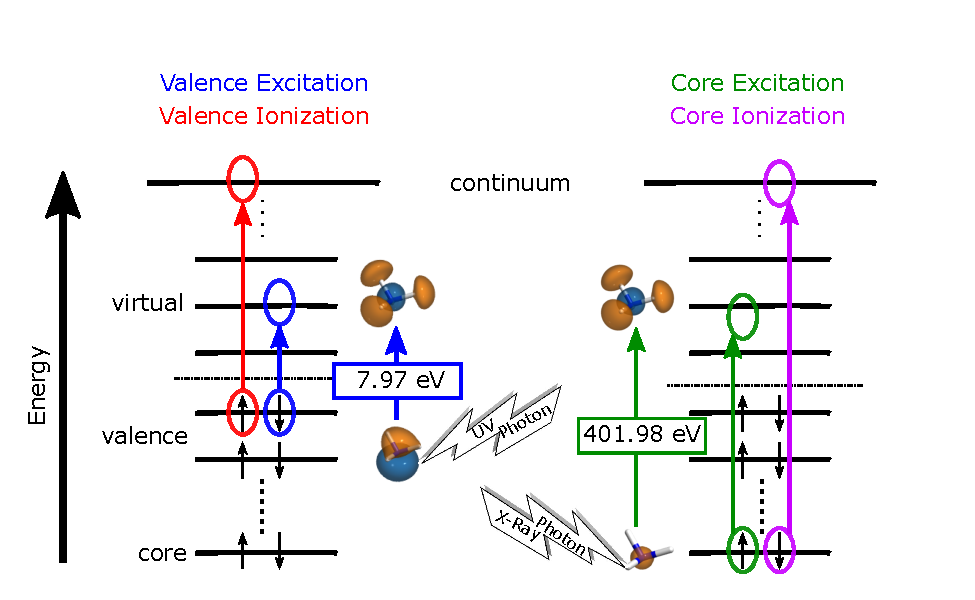
\includegraphics[scale=0.7]{photochem_graphic.pdf}
\caption{Sketch of the difference between UV and X-ray photo-absorption. The energies are not true to scale. The valence excitation and valence ionizaton processes are shown in blue and red respectively. The core excitation and core ionization processes are shown in green and purple respectively. An example is shown of the first valence and core excited state in ammonia (NH$_3$), the orbitals shown are hole and particle from orthogonality constrained density functional theory excited state computations at the B3LYP/3-21G level of theory.}
\label{fig:photochem}
\end{figure}

When a molecule is not under the influence of any external radiation it is in its ground electronic state (S$_0$). Photons from impending radiation can excite the molecule from the ground state to an electronic excited state, promoting an electron from an occupied molecular orbital (MO) to a higher energy unoccupied MO (often referred to as a ``virtual'' orbital in quantum chemistry). The excitation energy ($\omega$) of the electronic excited state will depend upon the energy of the impending radiation. The lifetime of these electronic excited states are extremely quick compared to the lifetime of molecular vibrations and thus these states can often be modeled properly within the vertical Franck-Condon approximation \cite{franck_elementary_1926,condon_theory_1926,condon_nuclear_1928,hazra_first_2004} where the electronic transition is assumed to occur without significant changes to the positions of the nuclei of the molecular system. The molecule eventually relaxes back down to its ground state level via a subsequent decay process such as fluoresence, \cite{maxwell_chlorophyll_2000,valeur_molecular_2012} phosphorescence, \cite{tanaka_observation_2005,romanovskii_phosphorescence_2000,cavar_fluorescence_2005} non-radiative relaxation, \cite{callomon_non-radiative_1972,de_mello_donega_non-radiative_1995} intersystem crossing, \cite{lamola_mechanisms_1965,hauser_intersystem_1991} and a myriad of other processes. \cite{zakrzewski_threshold_1984,meskers_relaxation_2000,vant_hof_zero-field_1976,hors_cross-relaxation_1982}

A unique class of electronic photo-excitations involves promotion of a core electron to a valence MO, this is referred to as a core excited state. The electrons that constitute the ``core'' of a molecule are those occupying the lowest molecular orbitals. The number of MOs that compose the core is dependent upon the atomic number ($Z$) of the atom involved. For example, for lighter first-row elements in the periodic table, like oxygen, the 1s orbital is the only core orbital. However, for heavier elements, the 2s and 2p are also apart of the core. For transition metals, like titanium the core also includes the 3d electrons that are crucial to metal bonding. Due to the strong Coulombic attraction of these electrons to the nuclei, a large amount of energy is required in order to promote an electron from this core level. Thus while ultraviolet (UV) or visible (VIS) photons are sufficient to liberate valence electrons, high energy X-ray photons are required in order to liberate core electrons. If the energy of the X-ray photon is greater than the core electron binding energy (CEBE) for a respective core electron then it creates a core excited state. Figure \ref{fig:photochem} details this process for both the valence and core cases respectively where the ionization process is defined as an electron being promoted from its occupied MO to the continuum.

The study of core-valence excitations caused by interactions of X-rays with molecules and the resulting spectra they produce is known as X-ray absorption spectroscopy or XAS. [CITE] XAS is a rapidly growing field that has matured significantly over the last few decades thanks to advances in synchrotron radiation technology. [CITE] Synchrotrons produce an intense tunable x-ray beam that can be used to scan a wide energy range throughout the x-ray region. Due to the large degree of energetic separation between the core and valence region, the spectrum produced by core-valence excitations has a prominent spike. This spike in the spectrum is known as the absorption ``edge'' and corresponds to the energy at which the X-ray photon is equal to the CEBE of the core electron. A unique edge feature is produced depending upon the principal quantum number of the associated core orbital with the K-edge referring to excitations from the 1st shell, the L-Edge referring to excitations from the 2nd shell, etc. Since the CEBE is largely dependent upon the charge of the nuclei, X-ray absorption techniques are element specific yielding a distinct signal for every atomic center in the molecule. For example, the K-edge of oxygen is located at approximately 530 eV while the K-edge for nitrogen is located at approximately 400 eV. The K-edge spectrum is rich with fine structure and can be divided into three distinct regions based on proximity to the absorption edge: the pre-edge, the near-edge, and the extended edge feature. The pre-edge feature is typically located at 10+ eV lower energy than the absorption edge. Core transitions to unoccupied 3d orbitals produce the most prominent features in the pre-edge region and thus, this region is mostly found in the K-edge spectra of transition metal complexes. [CITE] However other systems that form coordinated complexes also show some pre-edge features such as hydrogen bonded water complexes. [CITE] The near-edge region refers to any contributions along the ``rising edge'' of the edge feature. This region of the spectrum is populated by core transitions to virtual MOs of $\pi^*$ or $\sigma^*$ character and is present in any K-edge spectrum. Once the core electron reaches the continuum region, the electron can act as a free De Broglie wave and interact with the surrounding environment, the constrictive and destructive interference of the electron with the surrounding environment produces the features seen in the extended edge region. Each of these regions of the spectrum unveil different information regarding molecular electronic structure, the next sections will further reveal the usefulness of each region of the spectrum and show examples of their utility in electronic structure theory. 
\subsection{Theoretical Approaches for Calculation of Core Excited States}
A significant amount of progress has been made over the last few decades in order to make computations of core-excited states feasible and efficient in a plethora of different theories in quantum chemistry. As synchrotron facilities have become more powerful and plentiful the amount of high-quality X-ray absorption data has grown exponentially, inspiring more development in theory. Most modern techniques for the treatment of core-excitations fall into one of five classes that will be reviewed here: Hartree--Fock Static Exchange (HF-STEX), core valence separation (CVS), restricted excitation window (REW), energy specific (ES), or complex polarization propagator (CPP) methods. This review will focus primarily on methods used routinely in K-edge applications, there are more detailed multi-reference and relativistic methods in order to accurately treat the L-edge however those methods are outside the scope of this thesis. 
\subsection{Hartree-Fock Static Exchange}
HF-STEX (also known as improved virtual orbital Hartree--Fock) is a state specific approach in which the excited states are classified based on the atom-centered location of the core-hole. Within this theory, the final excited state characterized by the promotion of a core electron from the occupied space to the virtual space. The energy of the (N-1) state is calculated self-consistently and includes direct relaxation of the orbitals within the field of the core-hole potential. This direct inclusion of relaxation effects is one of the strongest advantages of HF-STEX based methods and is the starting approximation for practically every state specific/variational approach for core-excited state. The validity of this approximation supported by the large energy separation between the core and valence orbitals as well as the spatial separation of core orbitals on different atomic centers within a molecule.  

HF-STEX can be best understood as an approximate solution to the random phase approximation (RPA).  Lets consider a general RPA excitation operator $\hat{T}_I$ for an excited state $I$ within the Tamm-Dancoff approximation (TDA):
\begin{equation}
\hat{T}_I = \sum_{i,a} (\mathbf{X}_{ia,I}\hat{a}^{\dagger}_{a}\hat{a}_i)
\end{equation}
where $\mathbf{X}$ is the eigenvector of the RPA equation within the TDA, while $i$ and $a$ are indices that run over the ground state occupied and virtual orbitals respectively. This type of excitation operator contitutes what's known as a ``multi-channel'' approach, essentially a linear combination of single excitations that accounts for the interaction of different excitation channels. For HF-STEX, this excitation operator is limited to a restricted sum over single excitations from a given orbital $j$, this is also known as a ``single-channel'' approach
\begin{equation}
\hat{T}_I = \sum_{a} (\mathbf{X}_{ja,I}\hat{a}^{\dagger}_{a})\hat{a}_j
\end{equation}
It should be noted that this would be an extremely poor approximaton for a UV spectrum of valence excitations as multiple excitation channels tend to be clustered within a fairly small energy range (potentially less than 1 eV). However, due to the large energy separation of core orbitals, it is possible to obtain an accurate simulation of the XAS spectrum within a single channel approximation. Considering an excitation from core orbital $j$ to valence orbital $b$ from a closed shell reference state $|\Psi_0\rangle$, the STEX eigenvalue problem can be defined as
\begin{equation}
\label{eq:HFSTEX_eig}
F^j \phi_b = \epsilon_{jb} \phi_b,
\end{equation}
where $F^j$ is the HF-STEX Fock operator
\begin{equation}
F^j = h + \sum_{i \neq j} (2J_i - K_i) + J_j + K_j.
\end{equation}
the excitation energy ($\omega_{jb}$) are then obtained by adding the core ionization potential to the eigenvalue obtained in Equation \ref{eq:HFSTEX_eig}. The oscillator strengths are evaluated in terms of the excitation energy and the transition dipole moment as
\begin{equation}
f_{jb} = \frac{2}{3} \omega_{jb}|\langle \Psi_0|\vec{r}|\Psi_{jb}\rangle|^2
\end{equation}
With regard to the performance of HF-STEX, it produces XAS spectra that are in acceptable quantitative agreement with experimental results. HF-STEX oscillator strengths also provide a good qualitative comparison with experimental line intensities. These attractive features of the theory are however hampered by two main problems with the theory.  The first is the difficulty of converging an SCF solution with an empty core-hole. These states are notoriously difficult to converge suffering from the problem of variational collapse, and with multiple calculations necessary to simulate a full NEXAFS spectrum, this issue can be crippling. Work by Peter Gill has made strides toward alleviating this difficulty by employing a maximum overlap method (MOM) for excited states which works well for many cases however is not guaranteed to overcome variational collapse issues. The second challenge with HF-STEX lies in the non-orthogonality of the excited states within the core-hole potential. These two issues are crucial for all variational excited state methods applied to core-excitations and become the main motivation behind the work in this thesis. 

\subsection{Coupled Cluster Approaches}
The coupled-cluster wavefunction ($\Psi_{\rm CC}$) can be defined as an exponential expansion of a closed 
shell HF reference ($\Psi_{\rm HF}$)
\begin{equation}
|\Psi_{\rm CC}\rangle = e^{\hat{T}}|\Psi_{\rm HF} \rangle
\end{equation}
where $\hat{T}$ is known as the cluster operator and is composed of cluster amplitudes ($t_{\mu}$) and excitation operators ($\tau_{\mu}$)
\begin{equation}
\hat{T} = \sum_{\mu} t_{\mu} \tau_{\mu}
\end{equation}
The energy and amplitudes of the ground state can then be determined by projections onto the reference state and onto a manifold of excitations outof the reference state
\begin{align}
E &= \langle \Psi_{\rm HF} | e^{- \hat{T}}H e^{\hat{T}} |  \Psi_{\rm HF} \rangle \\
\Omega_{\mu} &= \langle \Psi_{\mu} | e^{- \hat{T}}H e^{\hat{T}} |  \Psi_{\rm HF} \rangle = 0
\end{align}
Within coupled-cluster theory, excited states can be obtained via a linear-response approach as well as a state-specific approach. Both approaches have challenges that must be overcome in order to calculate core-excited states. These methods for calculating core-excited states will be reviewed here.
\subsubsection{Linear-Response Coupled Cluster Theory}
Within coupled-cluster linear response theory, excitation energies ($\omega_{k}$) are obtained by solving an asymmetric eigenvalue equation to obtain right ($\mathbf{R}_k $) and left ($\mathbf{L}_k$) eigenvectors, commonly referred to as excitation and de-excitation operators respectively
\begin{align}
\label{eq:right_cc}
\mathbf{AR_k} &= \omega_k \mathbf{R_k} \\
\label{eq:left_cc}
\mathbf{L_kA} &= \omega_k \mathbf{L_k}
\end{align}
where the left and right eigenvalues are orthogonal ($\mathbf{L_iR_k} = \delta_{ik}$), and A is a Jacobian matrix that is defined as the gradient of the cluster amplitudes
\begin{equation}
A_{\mu \nu} = \frac{\partial \Omega_{\mu}}{\partial t_\nu}
\end{equation}
Many general schemes to iteratively solve Equations \ref{eq:right_cc} and \ref{eq:left_cc} have been introduced for excited state calculations. [CITE] These methods typically rely on using HF orbital energy differences to select guess unit vectors for specific occupied to virtual excitations. One fatal flaw that many methods encounter when trying to calculate core-excitations, is that the iterative solver will converge onto the lowest energy eigenvalues and eigenvectors even if the starting unit vectors are chosen for higher energy excitations. To overcome this difficulty, Sonia Coriani and Henrik Koch introduced a novel approach to iteratively solving Equations \ref{eq:right_cc} and \ref{eq:left_cc} using an asymetric Lanczos algorithm. This approach employs a tridiagonal representation $\mathbf{T}$ of the Jacobian matrix $\mathbf{A}$. 
\begin{equation}
\mathbf{T} = \mathbf{P^T A Q}
\end{equation}
where $\mathbf{P^TQ} = \mathbf{1}$. The diagonalization of $T$ is truncated at a dimension that is greatly reduced compared to the full dimension of possible excitations, generating an effective excitation spectrum. Using this approach the excitation spectrum converges to the exact excitation spectrum from the bottom or the top, i.e. higher energy starting vectors do converge on the higher energy. 
\subsubsection{Equation-of-Motion Coupled Cluster Singles and Doubles}
Within the framework of Equation-of-motion (EOM) CCSD the left ($\mathbf{L}$) and right ($\mathbf{R}$) eigenvectors shown in Equations \ref{eq:right_cc} and \ref{eq:left_cc} are truncated to second-order. Within the context of EOM-CCSD, it is conveniant to define a normal ordered Hamiltonian ($H_N$) that can be defined as
\begin{equation}
H_N = e^{-T}He^T - E
\end{equation}
this normal ordered Hamiltonian is then used to build the matrix elements of the EOM-CCSD Hamiltonian 
\begin{align}
\nonumber
H_{\rm EOM-CCSD} &= 
\begin{bmatrix}
H^{\rm SS} & H^{\rm SD} \\
H^{\rm DS} & H^{\rm DD}
\end{bmatrix} \\
\nonumber
H^{\rm SS} &= \langle \Phi_{i}^{a} | H_N | \Phi_{k}^{c} \rangle \\
\nonumber
H^{\rm SD} &= \langle \Phi_{i}^{a} | H_N | \Phi_{kl}^{cd} \rangle \\
\nonumber
H^{\rm DS} &= \langle \Phi_{ij}^{ab} | H_N | \Phi_{k}^{c} \rangle \\
H^{\rm DD} &= \langle \Phi_{ij}^{ab} | H_N | \Phi_{kl}^{cd} \rangle
\end{align}
where $|\Phi_{i}^{a} \rangle$ and $|\Phi_{ij}^{ab} \rangle$ are the singly and doubly excited determinants respectively. This EOM-CCSD Hamiltonian is then diagonalized using a modified Davidson algorithm to obtain the excitation energy eigenvalue spectrum. Similar to CC-LR, EOM-CCSD suffers from a feasibility problem as the high energy core-excited states can only be obtained after first obtaining a series of lower energy solutions. The need to solve for the full dimension of excitations in order to reach the core-excited states of interest causes standard diagonalization techniques to become computationally expensive for all cases and impossible for reasonably large cases.
\subsection{Linear Response Time-Dependent Density Functional Theory Approaches}
With regard to computational cost, linear response time-dependent density functional theory (TDDFT) remains one of the most attractive options for calculating electronic excited states in a wide variety of systems. Within TDDFT, excitation energies ($\omega$) are calculated via solutions to the following non-Hermitian eigenvalue equation:
\begin{equation}
\label{eq:tddft_eigenvalue_equation}
\begin{pmatrix}
\mathbf{A} & \mathbf{B} \\
\mathbf{B^{\dagger}} & \mathbf{A^{\dagger}} 
\end{pmatrix} 
\begin{pmatrix}
\mathbf{X}\\
\mathbf{Y}
\end{pmatrix}
= \omega
\begin{pmatrix}
\mathbf{1} & 0 \\
0 & -\mathbf{1}
\end{pmatrix}
\begin{pmatrix}
\mathbf{X} \\
\mathbf{-Y}
\end{pmatrix}
\end{equation}
where the matrices $\mathbf{A}$ and $\mathbf{B}$ are given by
\begin{align}
\label{eq:A_matrix}
A_{ai\sigma,bj\tau} &=  \delta_{ij} \delta_{ab} \delta_{\sigma\tau}(\epsilon_{a\sigma} - \epsilon_{i\tau}) + (ia\sigma|jb\tau) + (ia\sigma|f_{\rm XC}|jb\tau) \\
\label{eq:B_matrix}
B_{ai\sigma,jb\tau} &= (ia\sigma|jb\tau) + (ia\sigma|f_{\rm XC}|jb\tau)
\end{align}

for occupied orbitals $i,j,...$, virtual orbitals $a,b,...$, spin indices $\sigma$ and $\tau$, and energy eigenvalues $\epsilon$. The second term in Equation \ref{eq:A_matrix} is the two-electron integral and can be expressed explicitly in terms of a set of Kohn--Sham orbitals ($\phi_i$) as:

\begin{equation}
(ia\sigma|jb\tau) = \int \int \phi^*_{i\sigma}(\mathbf{r}_1)  \phi^*_{a\sigma}(\mathbf{r}_1) \frac{1}{R_{12}} \phi^*_{j\tau}(\mathbf{r}_2) \phi^*_{b\tau}(\mathbf{r}_2) d\mathbf{r}_1 d\mathbf{r}_2
\end{equation}

while the third term is what is known as the exchange correlation kernel which can be expressed as the second-derivative of the spin densities $\rho_{\sigma}$ and $\rho_{\tau}$

\begin{equation}
(ia\sigma|f_{\rm XC}|jb\tau) = \int \phi^*_{i\sigma}(\mathbf{r}_1)  \phi^*_{a\sigma}(\mathbf{r}_1) \frac{\partial^2 E_{XC}}{\partial \rho{\sigma}(\mathbf{r}_1 \partial \rho_{\tau}(\mathbf{r}_2)} \phi^*_{j\tau}(\mathbf{r}_2) \phi^*_{b\tau}(\mathbf{r}_2) d\mathbf{r}_1 d\mathbf{r}_2
\end{equation}
where $E_{\rm XC}$ is the exchange correlation functional. Within the Tamm-Dancoff approximation (TDA) [CITE], Equation \ref{eq:tddft_eigenvalue_equation} reduces to a Hermitian eigenvalue equation $\mathbf{A}\mathbf{X} = \omega\mathbf{X}$. Eliminating the off diagonal elements $\mathbf{B}$ greatly reduces the computational cost of solving the equation and makes the theory formally similar to configuration interaction singles. Many modern implementations of TDDFT make use of some form of the Davidson algorithm which is a bottom up algorithm, i.e. one in which the lowest eigenvalues are obtained first. This is a reasonable and efficient choice when the excitations of interest are valence excitations. However, excitations involving the lower energy core orbitals introduce a significant computational challenge since there is typically a plethora of valence excitations below the target core excitations. Making the algorithm prohibitively expensive since it requires the full excitation matrices to be formed and subsequently diagonalized. Overcoming this prohibitive expense is the primary motivation of methods developed to calculate core excitations within the TDDFT. 
\subsubsection{Restricted Excitation Window TDDFT}
Originally proposed by Stener et al. [CITE], restricted excitation window TDDFT (REW-TDDFT) is a modification to the standard TDDFT algorithm that only allows electrons to be excited from a subset of core orbitals. This approximation is physically motivated by the large energy separation of core levels of different atomic species, and the large spatial separation of core orbitals on different atoms. This is normally done in one of two ways: (1) Core orbitals of interest are selected directly via orbital localization schemes for equivalent atoms [CITE] (i.e. selecting all MOs that have primarily oxygen 1s character) or (2) Use an orbital energy (energy difference) cutoff in order to filter out any orbitals (orbital pairs) that lie above (below) the user provided energy threshold. The latter option is by far the most popular and has become commonplace for TDDFT implementations in modern quantum chemistry packages. [CITE] 

Although REW-TDDFT allows for the computation of core excited states, it naturally inherits the issues of standard TDDFT calculations, namely the large dependence on the choice of exchange-correlation functional. This has lead to development of a new class of functionals for use with REW-TDDFT known as short range corrected (SRC) functionals which are modified versions of long range corrected (LRC) functionals used for charge transfer excitations in TDDFT. The LRC exchange correlaton functional can be expressed as
\begin{equation}
E^{\rm LRC}_{\rm XC} = E^{\rm SR-DFT}_{\rm X} + E^{\rm LR-HF}_{\rm X} + E^{\rm DFT}_{\rm C} 
\end{equation}
combining a DFT exchange in the short-range, with Hartree--Fock exchange in the longer-range. SRC functionals modify this general form to include a certain portion of Hartree--Fock exchange in the short range as well.
\begin{equation}
E^{\rm SRC}_{\rm XC} = c_{\rm X}E^{\rm SR-HF}_{\rm X} + E^{\rm SR-DFT}_{\rm X} + E^{\rm LR-HF}_{\rm X} + E^{\rm DFT}_{\rm C} 
\end{equation}
where $c_{\rm X}$ is a parameter that can be optimized. The major drawback with this method is that the amount of HF exchange in the functional must be re-optimized for any given situation which can be cumbersome and limits its reliability when it is applied to novel problems. 
\subsubsection{Energy Specific TDDFT}
Starting from the non-Hermitian eigenvalue problem shown in Equation \ref{eq:tddft_eigenvalue_equation}, this form is often placed into the following Hermitian eignvalue problem
\begin{equation}
(\mathbf{A} - \mathbf{B})^{1/2} (\mathbf{A} +\mathbf{B}) (\mathbf{A} - \mathbf{B})^{1/2} \mathbf{T} = \omega^2 \mathbf{T}
\end{equation}
where $\mathbf{T} = (\mathbf{A} - \mathbf{B})^{-1/2} |\mathbf{X} + \mathbf{Y} \rangle$. Energy Specific TDDFT (ES-TDDFT) aims to solve this Hermitian eigenvalue problem utilizing a ``growing window'' algorithm that starts from a set of trial vectors $\mathbf{C}$ associated with orbital pairs whose orbital energy difference are above a given threshold. A subspace $\mathbf{\tilde{M}}$ is then created using the trail vectors,
\begin{align}
\mathbf{\tilde{M}}^+ &= \mathbf{C^T} (\mathbf{A} +\mathbf{B})\mathbf{C} \\
\mathbf{\tilde{M}}^- &= \mathbf{C^T} (\mathbf{A} -\mathbf{B})\mathbf{C} \\
\mathbf{\tilde{M}} &= (\mathbf{\tilde{M}} ^-)^{1/2} (\mathbf{\tilde{M}} ^+) (\mathbf{\tilde{M}}^-)^{1/2}
\end{align}
Direct diagonalization is performed only in the subspace $\mathbf{\tilde{M}}$, which generates a new set of eigenvalues $\tilde{\omega}$ and eigenvectors $\tilde{T}$. Only those eigenvectors associated with eigenvalues above the user defined threshold are kept. These eigenvectors are then projected back onto the full MO space in order to calculate a residual, any new eigenvectors with significant amplitude are then added as a trial vector for the next iteration (hence the term ``growing window''). A new subspace is constructed from the expanded trial space and the process continues self-consistently until the residual is below a user-defined threshold.

Since this method checks the risidual of the subspace against the full MO space the final results that are obatained are true solutions of the TDDFT equations. Similar to REW-TDDFT however, it inherits the inaccruacy and functional dependence of TDDFT for the calculation of core excited states.

\subsection{Real-Time Time-Dependent Density Functional Theory}
An alternative time-dependent density functional theory approach is real-time TDDFT (RT-TDDFT). In RT-TDDFT the density matrix is propagated in time utilizing the time dependent form of the Fock matrix. [CITE] This is done by solving the following equation of motion
\begin{equation}
\label{eq:real_time_EOM}
i \frac{\partial \mathbf{D}(t)}{\partial t} = [\mathbf{F}(t), \mathbf{D}(t)]
\end{equation}
where $\mathbf{D}(t)$ is the time dependent one-electron density matrix and $\mathbf{F}(t)$ is the time dependent Fock matrix which can be expressed in the following form for the case of hybrid exchange-correlation functionals
\begin{equation}
\label{eq:time_dependent_fock}
\mathbf{F}[\mathbf{D}(t)] = \mathbf{H}^{\rm core} + \mathbf{J}[\mathbf{D}(t)] + \alpha\mathbf{K}[\mathbf{D}(t)] + \beta \mathbf{E}_{\rm X}[\rho(\mathbf{r}, t)] + \gamma \mathbf{E}_{\rm C}[\rho(\mathbf{r}, t)] - \mathbf{\mu} \mathbf{V}^{\rm ext}(t)
\end{equation}
where $\rho(\mathbf{r}, t)$ is the time-dependent electron density, $\mathbf{\mu}$ is the dipole matrix, and $\mathbf{V}^{\rm ext}(t)$ is the applied external potential. The coefficients $\alpha$, $\beta$, and $\gamma$ are parameters that control the amount of Hartree--Fock and DFT exchange respectively. It should be noted that the expression in Equation \ref{eq:time_dependent_fock} only considers the coupling of the dipole moment with the external potential, this is valid within the ``long wavelength'' approximation where it is assumed that the photon is much longer than the system size. This approximation is almost always valid for UV/Vis photons and X-ray photons of organic molecules, however it can breakdown for higher energy core excitations in transition metals. At which point it will be necessary to consider higher order multipole moments beyond the electric dipole approximation. [CITE]

Solutions to the real-time approach involve integrating Equation \ref{eq:real_time_EOM} in order to obtain the time-dependent density matrix.  The Magnus expansion is a popular integrator for obtaining these solutions, [CITE] within this expansion the density matrix is propagated through time via a unitary propagator which conserves idempotency. The exact unitary propagator for Equation \ref{eq:real_time_EOM} is given as
\begin{equation}
\mathbf{U}(t + \Delta t, t) = T \ {\rm exp}\{-i \int^{t+\Delta t}_t \mathbf{F}(\tau) d\tau\}
\end{equation}
such that the time propagation of the density matrix can be written as
\begin{equation}
\mathbf{D}(t + \Delta t) = \mathbf{U}(t + \Delta t, t) \mathbf{D}(t) \mathbf{U}^{\dagger}(t + \Delta t, t) 
\end{equation}
where $\Delta t$ is the time-step and $T$ is a time-ordering operator that orders the operations associated with later times from those associated with earlier times. Due to the explicit time dependence of the Fock matrix it is impossible to evalute this propagator directly. However, it can be written in terms of a Magnus expansion
\begin{equation}
 T \ {\rm exp}\{-i \int^{t+\Delta t}_t \mathbf{F}(\tau) d\tau\} = e^{\Omega_1 + \Omega_2 + ... +\Omega_M}
\end{equation}
where $M$ is the total number of Magnus terms $\Omega_i$. The Magnus expansion is typically truncated at $M=1$ such that the unitary propagator can be approximated as
\begin{align}
\mathbf{U}(t + \Delta t, t) &\approx e^{\Omega_1} \\
\Omega_1 &\approx -i\mathbf{F}(t + \Delta t/2)
\end{align}
Within this form, the Fock matrix at a future time is guessed via linear extrapolation and solved for iteratively. This allows for the following explicit form of the time propagation of the density matrix
\begin{equation}
\mathbf{D}(t + \Delta t) = e^{-i\mathbf{F}(t+\Delta t/2)\Delta t} \mathbf{D}(t) e^{-i\mathbf{F}(t+\Delta t/2)\Delta t} 
\end{equation}
Core excitations typically have oscillations on the attosecond timescale, thus time steps on the tenth of an attosecond time scale must be taken to ensure accuracy within this region. An optical absorption spectrum can be obtained from a real-time simulation via a Fourier transform of the time-dependent dipole moment that results from a small applied electric field. For excitations on longer time scales a Gaussian electric field can be chosen, however to accomodate the short time scales of core excitations a delta function perturbation is typically applied [CITE]
\begin{equation}
\mathbf{E}_{\delta}(t) = \kappa \delta(t) \mathbf{\hat{d}}
\end{equation}
%\subsection{Theoretical Treatment of X-Ray Absorption Spectroscopy}
%Our starting point for an introduction to the theory of XAS is the simplification of the many electron problem into a generalized independent particle approximation based on the standard hole/electron quasiparticle picture. This simplifies the many-body theory into an effective independent electron approximation of an electronic excitation from initial state $|i\rangle$ to final state $|f\rangle$. Within this simplified picture, the absorption coefficient $\mu$ for a given photon energy $\omega$ can be expressed as
%\begin{equation}
%\mu(\omega) \approx \sum_f | \langle i | d | f \rangle |^2 \delta(\hbar \omega + E_i - E_f)
%\end{equation}
%where $\hbar \omega + E_i$ is the energy of the photoelectron and $d$ is the dipole coupling to the x-ray field. This equation is essentially a sum over final states $|f\rangle$. The composition of the final states are important to the theory and must provide an accurate representation of the excited state, however their construction in this case is not obvious. Many modern one-electron theories construct the final states in a self-consistent potential that includes a core-hole, this procedure is known as the Hartree--Fock static exchange approximation (HF-STEX). This approximation is physically motivated by the large energy separation of core levels of different atomic species, and the large spatial separation of core orbitals on different atoms. Allowing for a single excitation to be modeled in terms of relaxed orbitals from a given core-hole state. Within this approximation, $\psi_f$ is the wavefunction representing the final state with $h^{\prime}$ as the Hamiltonian of the core-hole potential, yielding the following eigenvalue equation
%\begin{equation}
%h^{\prime} \psi_f = E \psi_f
%\end{equation}
%where E represents the final state energies, and $h^{\prime}$ has the following form
%\begin{equation}
%h^{\prime} = \frac{p^2}{2m} + V^{\prime}_H + \sum(E)
%\end{equation}
%where the first term is the kinetic energy, $V^{\prime}_H$ is the Hartree potential of the core-hole state and $ \sum(E)$ is the self-energy term. This quantity is a complex valued, dynamically screened exchange interaction that accounts for the many body effects of extrinsic loses that occur due to the propagation of the photoelectron. $ \sum(E)$ is analogous to the exchange correlation potential of density functional theory, essentially containing all information not captured in the kinetic and potential term. Within GW theory, $ \sum(E)$ has been effectively approximated and provides accurate results for EXAFS spectroscopy. However, this term is overestimated for near-edge applications and thus further treatment is necessary.
%\subsection{Near-Edge X-ray Absorption Fine Structure}
%As with any form of photo-electron spectroscopy the interpretation of XAS spectroscopy relies on the Beer-Lambert law which relates the exponential decrease of the intensity ($I$) of the transmitted beam with respect incident beam intensity ($I_0$):
%\begin{equation}
%I = I_0 e^{-\mu D}
%\end{equation}
%where $D$ is the sample thickness and $\mu$ is what's known as the linear absorption coefficient which is related to the absorption cross-section, $\sigma_i$, of the $n$ unique chemical elements present in the sample
%\begin{equation}
%\mu = \frac{1}{V} \sum^n_{i = 1} \sigma_i
%\end{equation}
%where $V$ is the volume of the sample. Interpretation of the spectrum requires analysis of the position, intensity, and spape of peak features. As stated earlier, the position of peak features an energy specific signature of the absorbing atom. However, the technique is sensitive enough to differentiate between the same element in unique chemical environments.
%\begin{figure}
%\centering
%\includegraphics[scale=0.5]{chromium_k_edge.png}
%\caption{NEXAFS spectra at the Cr K-edge of four unique Cr(III) containing compounds. Experimental spectra are shown as solid lines, theoretical spectra are shown as dotted lines and are calculated using multiple scattering theory inside the FEFF8 code.[CITE] All data is from ref [CITE]}
%\label{fig:chromium_k_edge}
%\end{figure}
%For example, Figure \ref{fig:chromium_k_edge} shows the different spectra for four different Cr(III) containing metal complexes. Although all of the Cr K-edge spectra appear in the same region (5980 - 6050 eV), each unique complex has a different spectral profile in terms of peak positions and lineshapes. This shows that NEXAFS is sensitive to differences in the electronic structure, even the structurally similar CrF$_3$ and CrCl$_3$ have drastically different K-edge footprints. The same is true of atoms at different oxidation states, when increasing oxidation the edge tends to shift toward higher energy. This makes NEXAFS an excellent tool to check the valence state of atoms. 

%The K-edge, which consists of excitations of 1s electrons forms a rich structure for any atom that serves as a resource to interpret the unoccupied states of the electronic structure. The L-Edge is more complex to interpret, however is just as powerful in interpreting information about a molecules electronic structure. The complexity arises from the degeneracies that exist at the 2p electronic level, this introduces an element of strong electron correlation and causes splitting in the spectrum related to spin-orbit coupling between the occupied p-orbitals and unoccupied 3d states. 

\section{Orthogonality Constrained Density Functional Theory}
In this section, I review orthogonality constrained density functional theory (OCDFT) as a general approach to electronic excited states. OCDFT belongs to a unique class of density functional approaches whose main goal is to study excited states without using a time-dependent formulation, otherwise known as time independent density functional theory (TIDFT). [CITE] These methods provide an alternative to TDDFT which has been known to struggle in cases of charge transfer and Rydberg excited states due to inadequacies of approximate exchange correlation functionals. [CITE] 

OCDFT is a variational formulation of DFT for the calculation of excited states. Unique to the theory is the explicit enforment of constraints that guarantee orthogonality while allowing the MOs to fully relax. This draws inspriation from two TIDFT theories: 
\begin{itemize}
\item The variational TIDFT approach of Levy and Nagy which provides the theoretical framework for a universal excited state density functional,[CITE] thereby justifying the variational optimization of an excited state in DFT.
\item The constrained DFT (CDFT) approach of Van Voorhis and coworkers [CITE] which provides a framework for studying systems within Kohn--Sham DFT that have an arbitrary constraint on their density.
\end{itemize} 
The remainder of this section will provide a brief introduction to the theory, following this introduction will be a discussion of the features of the theory that specifically make it an attractive choice for the calculation of core-excited states.
\subsection{Original Formulation via Constrained Variational Minimization}
Within a generalized Kohn--Sham (KS) framework, an $n$-electron system can be represented in terms of an auxiliary system of noninteracting electrons. The KS auxiliary system can be represented by a single Slater determinant 
\begin{equation}
|\Phi\rangle = | \phi_1, \phi_2, ..., \phi_n \rangle
\end{equation}
which is constructed from a set of KS orbitals \{$\phi_i$\}. The total ground state electronic energy of the KS system can be expressed as
\begin{equation}
E_{\rm KS}[\{\phi_i\}] = - \frac{1}{2} \sum^{\rm occ}_i \langle \phi_i| \bigtriangledown^2 | \phi_i \rangle + \int d\mathbf{r} \nu(\mathbf{r}) \rho(\mathbf{r}) + J[\rho] + E_{\rm XC}[\rho]
\end{equation}
where the first term is the kinetic energy contribution, the second term is the contribution of the external potential, while $J[\rho]$ and $E_{\rm XC}[\rho]$ are the Coulomb and exchange-correlation contribution respectively. In general, an excited state can be computed by a constrained minimization of the expectation value of the Hamiltonian ($\hat{H}$) over all the wave funtions orthogonal to the ground state $\Psi$:
\begin{align}
E^{\prime} &= \min_{\rho^{\prime}}\left\{\min_{\substack{\Psi^{\prime} \rightarrow \rho^{\prime} \\ \Psi^{\prime} \perp \Psi}} \langle \Psi^{\prime}| \hat{H} | \Psi\rangle \right\} \\
&= \min_{\rho^{\prime}}\left\{ \int d\mathbf{r} \nu(\mathbf{r}) \rho(\mathbf{r}) + F^{\prime}[\rho^{\prime}]\right\}
\end{align}
where $F^{\prime}[\rho^{\prime}]$ minimizes the sum of the kinetric energy ($\hat{T}$) and electron-electron repulsion. In the spirit of the variational TIDFT of Levy and Nagy, OCDFT introduces a ficticious KS system of noninteracting electrons with density $\rho^{\prime}_s$ which maps to the excited state density of the real interacting system $\rho^{\prime}$ and can be described by a unique Slater determinant $\Phi^{\prime}$. The excited state solution is obtained via a \textit{constrained minimization} subject to an orthogonality constraint on the auxiliary wavefunctions
\begin{equation}
\langle \Phi^{\prime}|\Phi \rangle = 0
\end{equation}
Direct imposition of this orthogonality constraint avoids the excited state wavefunction from collapsing to the ground state solution. The OCDFT energy functional for the excited state is then expressed as
\begin{equation}
E^{\prime}_{\rm OCDFT}[\{\phi^{\prime}_i\}] = - \frac{1}{2} \sum^{\rm occ}_i \langle \phi^{\prime}_i| \bigtriangledown^2 | \phi^{\prime}_i \rangle + \int d\mathbf{r} \nu(\mathbf{r}) \rho^{\prime}(\mathbf{r}) + J[\rho^{\prime}] + E_{\rm XC}[\rho^{\prime}]
\end{equation}
Note that the exchange-correlation functional $E_{XC}$ is the same as the ground state functional only evaluated at the excited state density, this is an adiabatic approximation for the excited state and is discussed in more detail in Ref. [CITE]. 
\subsection{Attractive Features of OCDFT for Core Excitations}
This section will focus on the features of orthogonality constrained density functional theory that made it an attractive candidate as a theory to apply to core excitations. Three features stand out the most and will be covered in more detail in this section:
\begin{itemize}
\item Full inclusion of orbital relaxation effects through variational optimization of Kohn--Sham orbitals.
\item Variational stability of the $\Delta$SCF procedure due to imposition of orbital orthogonality.
\item Computational cost and scaling comparable to time-dependent density functional theory.
\end{itemize}
Having established itself as a stable, cheap, and accurate theory for electronic excited states the extension of this theory for the treatment of core excited states seemed like a logical progression.
\subsubsection{Orbital Relaxation Effects}
Due to the large amount of energy necessary to excite electrons occupying core orbitals to the virtual level, orbital relaxation effects begin to play a vital role. Core electrons have a strong attraction to the nucleus, thus its photoexcitation reduces the shielding of the nucleus and  causes significant rearrangement of the valence electrons. [CITE] Compared to excitations where the valence electron arrangement is fairly similar to the initial configuration, core excitations have a significant lowering of the total energy of the final state. [CITE] This effect becomes even more pronounced when more valence electrons are available meaning proper treatment of orbital relaxation is even more critical when considering core excitations of heavier elements. [CITE] 

Within OCDFT, a general excited state determinant $\Phi^{\prime}$ for an $n$-electron system is optimized with respect to a set of excited state orbitals $\{\phi_n^{\prime}\}$ 
\begin{equation}
|\Phi^{\prime} \rangle = | \phi^{\prime}_1, \phi^{\prime}_2, ..., \phi^{\prime}_n \rangle
\end{equation}
Since the excited state is variationally optimzed, relaxation effects are explicitly considered for each excited state determinant. Within a quasiparticle framework, two of the orbitals that compose this slater determinant will define the excitation process as the hole ($\phi^{\prime}_h$) and particle ($\phi^{\prime}_p$) respectively. The excited state orbitals are optimized subject to a set of minimal orbital orthogonality conditions: 1) The occupied orbitals are restricted to span the space complementary to the hole orbital 
\begin{equation}
\langle \phi^{\prime}_i|\phi_h^{\prime}\rangle = 0, i=1,2,...n
\end{equation}
and 2) The hole orbital must be constrained to span the occupied space of the ground state determinant $\Phi$. Optimizing the the excited state relative to these two constraints is sufficient to produce an orthogonal excited state solution. This formalism provides the flexibility to control the degree of optimization of the wavefunction, i.e. to control the amount of relaxation that it explicitly included in the calculation. This analysis was very useful for determining the importance of relaxation effects on the performance of OCDFT in valence excitations, [CITE] and a similar analysis is applied here to examine the importance for core excitations. We make use of 4 different levels of optimization 1) Obtaining the fully optimal hole/particle pair and allowing full relaxation of all alpha and beta orbitals 2) Obtaining the optimal hole/particle pair while only allowing relaxation of the alpha orbitals 3) Obtaining the optimal hole orbital only while allowing all other alpha/beta orbitals to relax and 4) obtaining the optimal particle only and allowing all other orbitals to relax. 
\begin{figure}
\centering
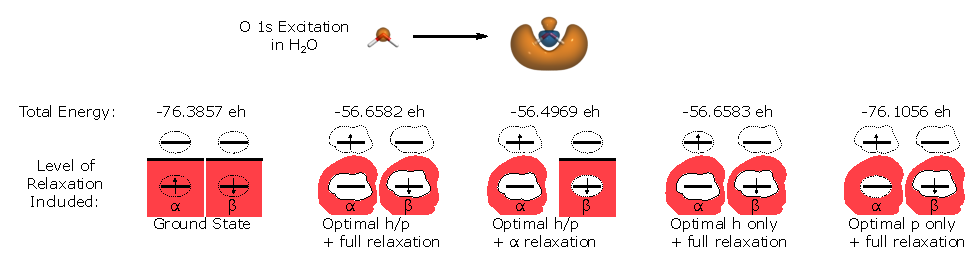
\includegraphics{h_p_algorithms.pdf}
\caption{First O 1s core excitation in H$_2$O calculated using orthogonality constrained density functional theory at the B3LYP/3-21G level of theory. Numbers reported are the total energy of the ground state and respective core excited state calculated with varying degrees of orbital relaxation included.}
\label{fig:relax}
\end{figure}
Figure \ref{fig:relax} shows the results of applying these different levels of relaxation to the first core excited state in H$_2$O. Optimizing the hole and particle pair with full relaxation yields a total energy of $- 56.6582$ Hartree. Only relaxting the $\alpha$ orbitals raises this energy by about 0.2 Hartree, showing that the rearangment that occurs in the electronic structure due to the creation of a core hole is significant. However, when only the particle orbital is optimized, the excited state energy lowers significantly to $-76.056$ Hartree. This shows that although valence rearrangement is ultimately important, inclusion of hole relaxation effects is the primary orbital relaxation contribution. The ability of OCDFT to explicitly account for this effect makes it an excellent method for computing core excitation energies accurately. 
\subsubsection{Stability of the Self-Consistent Algorithm}
The Ritz variational principle defines the energy expectation value $\tilde{E}$ of any trial wavefunction $\tilde{\phi}$ as an upper-bound with respect to the ground state energy $E_0$ of the system
\begin{equation}
\tilde{E} = \frac{\langle \tilde{\phi}| \hat{H} | \tilde{\phi}\rangle}{\langle\tilde{\phi}|\tilde{\phi}\rangle} \geq E_0.
\end{equation} 
However, the energy of a variationally computed excited state $E^{\prime}$ is no longer a valid upper bound of the ground state energy unless the trial wavefunction ($\tilde{\phi}$) is constrained to be orthogonal to all lower lying states of the same symmetry. In this regard, a standard $\Delta$SCF calculation of an excited state can be viewed as an unconstrained optimization, which in many cases guides the final optimized excited state solution to the ground state wave function. This is a well known optimization problem called ``variational collapse.'' Considering this issue, it is desirable to have a method that allows for the general variational calculation of an excited state without sacrificing the orthogonality of the computed excited state wavefunction to lower lying states of the same symmetry. Imposing orthogonality constraints into the variational procedure ensures the strict upperboundedness of the computed excited state energies, which ensures that the optimization will not suffer from variational collapse. This is the approach taken by orthogonality constrained density functional theory as well as the ``takes orthogonality constraints into account'' (TOCIA) method. Other methods such as Morokuma's electron-hole potential (EHP) method and the constricted variational DFT method (CV-DFT) of Ziegler and coworkers aim to avoid this optimization problem without imposing exact orthogonality and instead impose different variational constraints. Despite these differences, all of these methods revolve around the variational minimization a unique KS energy functional for the excited state determinant $\Phi^{\prime}$ that is different from the ground state reference $\Phi$. They do this explicitly by parametrizing the wavefunction using a generic determinant, this can be expressed as a unitary transformation of the ground state determinant
\begin{equation}
|\Phi^{\prime} \rangle = |\phi_1^{\prime}, \phi_2^{\prime}, ..., \phi_n^{\prime} \rangle = e^{\hat{A}}|\Phi\rangle
\end{equation}
where $\hat{A}$ is a one-particle anti-Hermitian operator. To impose an orthogonality condition on the excited state wavefunction ($\langle \Phi^{\prime}|\Phi\rangle$ = 0) OCDFT imposes the minimal orbital orthogonality constraints necessary to obtain an orthogonal solution. For example, to provide a description of the lowest excited state, the ground state HOMO ($\phi_n$) is simply constrained to be orthogonal to the excited state occupied orbitals ($\phi_i^{\prime}$) 
\begin{equation}
\langle \phi_n|\phi_i^{\prime} \rangle = 0, i = 1,2,...,n
\end{equation}
This constraint guarantees that the excited state determinant is orthogonal to the excited state, thus ensuring that the resulting optimization procedure does not suffer from variational collapse. 
\subsubsection{Favorable Computational Cost and Scaling}
A cheap computational cost and favorable scaling with respect to system size are extremely important features of OCDFT that allows for a wide range of potential applications for the method. Formally the cost of OCDFT is identical to that of a ground-state DFT computation which scales as $N^3$ for pure functionals and $N^4$ for hybrid functionals, where $N$ is the number of electrons in the system. This scaling with respect to system size is comparable to that of CIS and TDDFT which also scale as $N^4$, in which the bottleneck in those methods is the contraction of a transition density matrix with the two-electron integrals. This scaling is better than that of ADC(2) and excited state CC2 which scale as $N^5$. Unlike CIS and TDDFT, OCDFT maintains this favorable cost while still obtaining accurate excitation energies comparable to more expensive methods, as will be shown in Chapters 2 and 3 of this dissertation.
\subsection{Prospectus}
In Chapter 2, we report an extension of orthogonality constrained DFT to compute core excited states and generalize the original formalism in order to calculate multiple excited state solutions. This chapter focuses on benchmarking the method with respect to experimental core excitation energies and simulating full experimental spectra. Chapter 3 reports the combination of OCDFT with a novel implementation of the spin-free exact-two-component (X2C) one-electron treatment of scalar relatavistic effects in order to study the importance of relativistic effects on core-excited states and treat K-edges of transition metal complexes. Chapter 4 describes a new technique for the automated classification of core excited states that utilizes a unique representation of the unoccupied orbitals known as the localized intrinsic valence virtual orbitals (LIVVOs). This new method of classification is integrated with the OCDFT hole/particle orbital formalism here. Chapter 5 deals with the unique case of targeting the K-edge chemisorbed organic molecules. We introduce a subspace projection algorithm into OCDFT in order to specifically target the core excitations of the organic adsorbate, which is not feasible in the bottom-up algorithm described in Chapter 2.
\bibliography{introduction}
\bibliographystyle{rsc}
\end{document}
